\section{Adaptive Color-to-Binary Decomposition Algorithms}
\label{sec:volumetric:acd}

In this section, we present methods for more efficient decomposition from color-volume to binary-volume, efficiency here referring to the number of binary depth planes that are used to represent a color depth plane. 

\subsection{Motivation}
\begin{figure}[!htb]
\centering
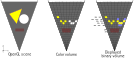
\includegraphics[width=0.99\columnwidth]{images/volumetric/adaptive_color_decomposition}
\caption[Volumetric NED: Motivation for adaptive color-to-binary decomposition]{Figure shows a concept diagram for adaptive color-to-binary decomposition. Note how the LED values written on the left side of the binary volume in this figure do not follow a repeating pattern as shown in Fig.~\ref{fig:volumetric:binary_decomposition}}
\label{fig:volumetric:acd}
\end{figure}


In the method presented in Sec.~\ref{sec:volumetric:fixed_pipeline}, each color voxel was decomposed into the nearest 24 binary depth planes. 
Since our display's LEDs can change color and intensity over a very large range on a per-binary frame basis, we don't need to limit our display to a fixed pattern of LED colors and intensities or to 8 bits-per-color. 
A more optimum decomposition method might use a fewer number of binary voxels to represent the same color voxel. 
Fig.~\ref{fig:volumetric:acd} shows a conceptual diagram of how the resulting binary volume of such adaptive color-to-binary decomposition algorithms may look.
It is useful to reduce the number of binary voxels that represent each color voxel for the following reasons:

\begin{enumerate}
    \item This will reduce the depth-blur associated with each color voxel.
    \item This may be useful for more compact prototypes because the more compact DMD projectors have a slower refresh rate than the DMD projector used in our display.
    \item We may be able to achieve High Dynamic Range imagery.
    \item With fewer number of binary voxels representing each color voxel, we can represent objects that are transparent and closer to each other than with the fixed pipeline decomposition. With the fixed pipeline decomposition, we can not represent objects along the same depth that are closer than $3 \times \text{color bit-depth}$.
\end{enumerate}


\subsection{Approach}
The basic idea behind the color adaptive decomposition methods explored here is that of error propagation or diffusion. 
Starting at the nearest depth plane, we consider the slice of the color volume and do the best of representing it with a binary image and an arbitrary LED color. 
Unavoidably, there will be errors, which are propagated onto the next depth plane. 
At the next depth plane, the current depth's slice of the color volume and the propagated errors are added and considered as the target image for the decomposition.
The pseudo-code for this approach is given in Algorithm.~\ref{alg:colorAdaptiveMethodOne}. 
\begin{algorithm}[!htb]
    \caption{Outline of error propagation appoach}
    \label{alg:colorAdaptiveMethodOne}
    \hspace*{\algorithmicindent}\textbf{Input:} Color Volume\\
    \hspace*{\algorithmicindent}\textbf{Output:} Binary Images, LEDs
    \begin{algorithmic}[1]
        \STATE{$\text{Residual} \gets \text{zeros}$}
        \FOR{$d \gets 1$ \TO $\numPlanes$}
        \STATE{Color Volume Slice $\gets$ Color Volume $\lbrack :,:,d \rbrack $}
        \STATE{Target $\gets$ Color Volume Slice $+$ Residual}
        \STATE{${(\text{Binary Image}_d, \text{LED}_d)} \gets \text{Decompose$(\text{Target})$}$}
        \STATE{$\text{Residual} \gets \text{Target} - \text{Reconstruct$(\text{Binary Image}_d, \text{LED}_d)$}$}
        \ENDFOR
    \end{algorithmic}
\end{algorithm}

\begin{comment}
\begin{algorithm}[!htb]
    \caption{Outline of error propagation appoach}
    \label{alg:colorAdaptiveMethodOne}
    \hspace*{\algorithmicindent}\textbf{Input:} $V$\\
    \hspace*{\algorithmicindent}\textbf{Output:} $B, L$
    \begin{algorithmic}[1]
        \STATE{$R \gets \text{zeros}$}
        \FOR{$d \gets 1$ \TO $\numPlanes$}
        \STATE{$I \gets V \lbrack :,:,d \rbrack $}
        \STATE{$T \gets I + R$}
        \STATE{${(B_d,L_d)} \gets \text{Decompose$(T)$}$}
        \STATE{$R \gets T - \text{Reconstruct$(B_d, L_d)$}$}
        \ENDFOR
    \end{algorithmic}
\end{algorithm}
\end{comment}

The methods explored here differ from each other in the way the target image at each depth is decomposed, i.e., the \emph{Decompose} function in Algorithm.~\ref{alg:colorAdaptiveMethodOne}.
In the sections below, we explore some possible ways to decompose the target image at each depth.
For each of the methods below, the decomposition step tries to minimize the L2-norm between the decomposition and the target images:
\begin{equation}
    \argmin_{\text{Binary Image}_d,\text{LED}_d} ||\text{Target} - \text{Reconstruct}(\text{Binary Image}_d, \text{LED}_d) ||^2
\end{equation}

However, the problem with trying to decompose a 24-bit target RGB image into a 1-bit DMD image and an RGB LED value is that:
\begin{enumerate}
    \item Because the DMD pattern is common for the three color channels, the decomposition is not separable among the color-channels, e.g., a particular DMD pattern may have a very low loss for the red channel but very high for the green channel such that the combined error might be lesser than completely leaving out the green channel. 
    \item Something to do with binarization. The threshold determines whether we under-expose or over-expose. When the decomposition under-exposes, the errors are propagated much farther away from the slice which caused the error.
    \item 
\end{enumerate}

\subsubsection{Combinatorial Optimization}
\label{sec:acd:combinatorial}
In this method, we calculate the decomposition for every combination of color channel. 
These are the difference combinations of color channels: $\text{Combination}_1 = $\{ 1, 0, 0 \}, $\text{Combination}_2 = $ \{ 0, 1, 0 \}, $\text{Combination}_3 = $ \{ 0, 0, 1 \}, $\text{Combination}_4 = $ \{ 1, 1, 0 \}, $\text{Combination}_5 = $ \{ 1, 0, 1 \}, $\text{Combination}_6 = $ \{ 0, 1, 1 \}, $\text{Combination}_7 = $ \{ 1, 1, 1 \}, where 0 indicates that the color channel is not considered for the optimization and 1 indicatest that the color channel is considered for the optimization. 

\begin{algorithm}[!htb]
    \caption{Combinatorial color decomposition}
    \label{alg:combinatorial}
    \hspace*{\algorithmicindent}\textbf{Input:} $\text{Target}, \text{Residual}$, \text{Color Volume Slice}\\
    \hspace*{\algorithmicindent}\textbf{Output:} $\text{Binary Image}, \text{LED}, \text{Residual}$
    \begin{algorithmic}[1]
        \STATE{$\text{Target} \gets \text{Color Volume Slice} + \text{Residual}$}
        \STATE{$ \{\text{Target}_R, \text{Target}_G, \text{Target}_B \} \gets \text{Split}(\text{Target})$}
        \FOR{$i \gets 1$ \TO $7$}
        \FOR{$j \gets \{R,G,B\}$}
        \IF{$\text{Combination}_i[j] == 0$}
        \STATE{$\text{LED}_j \gets 0$}
        \STATE{$\text{Binary Image}_j \gets I_{\text{ones}}$}
        \ELSE
        \STATE{$\text{LED}_j \gets \text{Mean}\left( \{ \text{Target}_j : \text{Target}_j \neq 0 \} \right)$}
        \STATE{$\text{Binary Image}_j \gets \text{Signum}\left( \frac{\text{Target}_j}{\text{LED}_j} - \text{Threshold} \right)$}
        \ENDIF
        \ENDFOR
        \STATE{$\text{Binary Image}_i \gets \text{Binary Image}_1 \odot \text{Binary Image}_2 \odot \text{Binary Image}_3$}
        \FOR{$j \gets \{R,G,B\}$}
        \IF{$\text{Combination}_i[j] == 0$}
        \STATE{$\text{LED}_j \gets 0$}
        \ELSE
        \STATE{$\text{Target}_j' \gets \text{Target}_j \odot \text{Binary Image}_i$}
        \STATE{$\text{LED}_j \gets \min \left( \{ \text{Target}_j' : \text{Target}_j' \neq 0 \} \right)$}
        \ENDIF
        \ENDFOR
        \STATE{$\text{LED}_i \gets \text{Combine}\left(\{\text{LED}_R, \text{LED}_G, \text{LED}_B \}\right)$}
        \STATE{$\text{Reconstruction}_i \gets \text{Reconstruct}(\text{Binary Image}_i,\text{LED}_i)$}
        \STATE{$\text{Residual}_i \gets \text{Target} - \text{Reconstruction}_i$}
        \STATE{$\text{Energy}_i \gets \text{Loss}(\text{Residual}_i)$}
        \ENDFOR
        \STATE{$k \gets \argmin(\text{Energy}_1,\text{Energy}_2,\ldots,\text{Energy}_7)$}
        \STATE{$\text{Binary Image} \gets \text{Binary Image}_k$}
        \STATE{$\text{LED} \gets \text{LED}_k$}
        \STATE{$\text{Residual} \gets \text{Residual}_k$}
    \end{algorithmic}
\end{algorithm}
\begin{comment}
\begin{algorithm}[!htb]
    \caption{Combinatorial color decomposition}
    \label{alg:combinatorial}
    \hspace*{\algorithmicindent}\textbf{Input:} $T, R$\\
    \hspace*{\algorithmicindent}\textbf{Output:} $B, L, R$
    \begin{algorithmic}[1]
        \STATE{$T \gets I + R$}
        \STATE{$ \{C_1, C_2, C_3 \} \gets \text{split}(T)$}
        \FOR{$i \gets 1$ \TO $7$}
        \FOR{$j \gets 1$ \TO $3$}
        \IF{$O_i[j] == 0$}
        \STATE{$L_j \gets 0$}
        \STATE{$B_j \gets I_{\text{ones}}$}
        \ELSE
        \STATE{$L_j \gets \mu\left( \{ C_j : C_j \neq 0 \} \right)$}
        \STATE{$B_j \gets \text{sgn}\left( \frac{C_j}{L_j} - T \right)$}
        \ENDIF
        \ENDFOR
        \STATE{$B_i \gets B_1 \cdot B_2 \cdot B_3$}
        \FOR{$j \gets 1$ \TO $3$}
        \IF{$O_i[j] == 0$}
        \STATE{$L_j \gets 0$}
        \ELSE
        \STATE{$C_j' \gets C_j \cdot B_i$}
        \STATE{$L_j \gets \min \left( \{ C_j' : C_j' \neq 0 \} \right)$}
        \ENDIF
        \ENDFOR
        \STATE{$L_i \gets \{L_r, L_g, L_b \}$}
        \STATE{$S_i \gets \text{Reconstruct}(B_i,L_i)$}
        \STATE{$R_i \gets T - S_i$}
        \STATE{$E_i \gets \text{Loss}(R_i)$}
        \ENDFOR
        \STATE{$k \gets \argmin(E_1,E_2,\ldots,E_7)$}
        \STATE{$B \gets B_k$}
        \STATE{$L \gets L_k$}
        \STATE{$R \gets R_k$}
    \end{algorithmic}
\end{algorithm}
\end{comment}
%\input{chapters/volumetric/algorithms/easy.tex}
See Algorithm~\ref{alg:combinatorial} for a pseudo-code for this approach. A step-wise explanation for the algorithm follows:
\begin{itemize}
    \item Lines 1-2: At each depth plane, we assign the target image by adding the previous residual to the current depth plane's image. We split this target image into its color channels because we process the color channel's independently in the initial part of the algorithm to estimate the common optimal binary image.
    \item Line 3: In the outer for-loop, we consider each of the seven possible options for whether an LED is on or off, i.e., $\text{Combination}_1$, $\text{Combination}_2$, ..., $\text{Combination}_7$, and save these calculated values: LED values, binary image, the reconstructed image, the residual, and the energy or loss.
    \item Lines 5-13: calculate the best LED value and binary pattern when each color channel is considered independently and in accordance with whether that color channel's LED should be on or off. If that color channel's LED should be off, then the LED value for that color channel is set to 0, and the binary pattern is set to all ones. If, however, the LED should be on, the LED value is calculated as the mean value of the non-zero pixel values of that color channel, and the binary pattern is calculated by thresholding the pixel values divided by the calculated LED value. Typically, this threshold is set to 1.
    \item Line 14: Since the DMD pattern is common to all three color channels, we need to calculate the common binary pattern by simply multiplying together all the color channel's binary patterns. 
    \item Lines 15-24: Because the common binary pattern may be different from each of the color channel's binary patterns, we need to calculate the new optimum LED values. This for-loop accomplishes that by assigning each LED value to the minimum pixel value in its color channel.
    \item Lines 27-30: We find which option resulted in the least energy and output that option's binary pattern, LED values, and residual image. 
\end{itemize}


\subsubsection{Highest Energy Channel Minimization}
\label{sec:acd:highestenergy}
\begin{algorithm}[!htb]
    \caption{Highest Energy Channel Minimization}
    \label{alg:highest_energy_channel_minimization}
    \hspace*{\algorithmicindent}\textbf{Input:} $\text{Target}, \text{Residual}$, \text{Color Volume Slice}\\
    \hspace*{\algorithmicindent}\textbf{Output:} $\text{Binary Image}, \text{LED}, \text{Residual}$
    \begin{algorithmic}[1]
        \STATE{$\text{Target} \gets \text{Color Volume Slice} + \text{Residual}$}
        \STATE{$ \{\text{Target}_R, \text{Target}_G, \text{Target}_B \} \gets \text{Split}(\text{Target})$}
        \STATE{$\{ \text{Energy}_R, \text{Energy}_G, \text{Energy}_B \} \gets \text{Loss}(\{ \text{Target}_R, \text{Target}_G, \text{Target}_B \})$}
        \STATE{$k \gets \argmin(\text{Energy}_R,\text{Energy}_G, \text{Energy}_B)$}
        \STATE{$\text{LED} \gets \{0, 0, 0 \}$}
        \STATE{$ \text{LED}_k \gets \text{Mean}(\text{Target}_k:\text{Target}_k \neq 0) $}
        \STATE{$\text{Binary Image} \gets \text{Signum}(\frac{\text{Target}_k}{\text{LED}_k} - \text{Threshold})$}
        \STATE{$\text{Reconstruction} \gets \text{Reconstruct}(\text{Binary Image},\text{LED})$}
        \STATE{$\text{Residual} \gets \text{Target} - \text{Reconstruction}$}
    \end{algorithmic}
\end{algorithm}

\begin{comment}
\begin{algorithm}[!htb]
    \caption{Highest Energy Channel Minimization}
    \label{alg:highest_energy_channel_minimization}
    \hspace*{\algorithmicindent}\textbf{Input:} $T, R$\\
    \hspace*{\algorithmicindent}\textbf{Output:} $B, L, R$
    \begin{algorithmic}[1]
        \STATE{$T \gets I + R$}
        \STATE{$ \{C_1, C_2, C_3 \} \gets \text{split}(T)$}
        \STATE{$\{ E_1, E_2, E_3 \} \gets Loss(\{ C_1, C_2, C_3 \})$}
        \STATE{$k \gets i:E_i = \max(E_1, E_2, E_3)$}
        \STATE{$L \gets \{0, 0, 0 \}$}
        \STATE{$ L_k \gets \mu(C_k:C_k \neq 0) $}
        \STATE{$B \gets \text{sgn}(\frac{C_k}{L_k} - T)$}
        \STATE{$S \gets \text{Reconstruct}(B,L)$}
        \STATE{$R \gets T - S$}
    \end{algorithmic}
\end{algorithm}
\end{comment}
See Algorithm~\ref{alg:highest_energy_channel_minimization} for a pseudo-code for this approach. A step-wise explanation for the algorithm follows:
\begin{itemize}
    \item Line 1: At each depth plane, we assign the target image by adding the previous residual to the current depth plane's image. 
    \item Line 2: Split the target image into its color channels because we process the color channel's independently.
    \item Line 3: Calculate the energy of each color channel.
    \item Line 4: Find the color channel that has the maximum energy. For the rest of the algorithm, it is only this color channel that is of interest to us. The other two color channels are ignored.
    \item Lines 5-6: Each LED color is first assigned to 0. Then, only for the color channel of maximum energy, the LED color is calculated as the mean of the non-zero pixel values of that color channel.
    \item Line 7: The binary image is calculated by thresholding the color channel of the maximum energy channel against the calculated LED color.
    \item Line 8-9: Calculating the reconstructed image and the residual image.
 \end{itemize}


\subsubsection{Projected Gradient}
\label{sec:acd:projected_gradient}
This approach is based on non-negative matrix factorization methods as used in recent compressive displays~\cite{Wetzstein2012,Huang2015Light,huang2017mixed}. 
However, the previous papers were concerned with decomposing a continuous-valued image into two or more continuous-valued images. 
Here, by continuous, we mean that the values are considered to be in continuous domain even through in a computer they may be represented by an 8-bit per color channel image. 
However, in our display, we need to decompose continuous-valued images (slices of the color volume) into a binary image and a continuous-valued triplet for the RGB LED. 
This is a significantly harder problem because it is a combination of the traditional optimization as explored by non-negative matrix factorization algorithms and combinatorial optimization which has not been investigated previously in the context of computational displays. 
In this section, we derive the update rules for non-negative matrix factorization algorithms, and we write down the algorithm and explain it.
We shall see later in the Sec.~\ref{sec:volumetric:acd:results} that this algorithm does poorly in terms of visual quality.

\paragraph{Newton's method adapted for optimization}
Non-negative matrix factorization's update rules can be understood from studying Newton's method adapted for optimization:

Taylor expansion:
\begin{equation}
  f(x) = f(x_0) + \Delta f'(x_0) + \frac{\Delta x^2 f''(x_0)}{2} + ...
\end{equation}
where $\Delta x = x - x_0$.

Let us consider only the first three terms of the Taylor expansion. We differentiate the above equation wrt $\Delta x$ to determine the optimum step size to guarantee fast convergence.

\begin{equation}
  \frac{d f(x)}{d(\Delta x)} = \frac{d \left( f(x_0) + \Delta f'(x_0) + \frac{\Delta x^2 f''(x_0)}{2}\right)}{d(\Delta x)} 
\end{equation}

\begin{equation}
  0 = f'(x_0) + \Delta x f''(x_0)
\end{equation}

Rearranging:
\begin{equation}
  \Delta x = - \frac{f'(x_0)}{f''(x_0)}
\end{equation}

Then,
\begin{equation}
  x_{n+1} = x_n - \frac{f'(x_0)}{f''(x_o)}
\end{equation}

\paragraph{Applying Newton's method for our problem}

This is the mathematics for the matlab file named \emph{adaptive\_color\_decomposition\_all\_channels.m}.

Now, let us apply Newton's method to our problem. Let us first denote the color volume by $V_c$, the
binary volume by $V_b$, the color sub-volume image to be $C$, the binary subvolume image to be
$B$, the LED color and brightness associated with $B$ to be $\alpha$. We now define the energy
function that is to be optimized:

\begin{equation}
  E = ||C - \alpha B||^2 = ||C^T - \alpha B^T||^2
\end{equation}

Note that the energy function is the L2-norm of the residual, $R$, defined as:
\begin{equation}
  R = C - \alpha B = C^T - \alpha B^T
\end{equation}

Deriving update rule for $B$
Expanding $E = ||C^T - \alpha B^T||^2$:
\begin{equation}
  E = C^TC - 2C^T\alpha B + \alpha^2 B^T B
\end{equation}

\begin{equation}
  \frac{dE}{dB} = -2\alpha C^T + 2\alpha^2 B^T
\end{equation}

and
\begin{equation}
  \frac{d^2E}{dB^2} = 2\alpha
\end{equation}

Then,
\begin{equation}
  \Delta B = \frac{2\alpha C^T - 2 \alpha^2 B^T}{2 \alpha^2} = \frac{C^T - \alpha B^T}{\alpha} = \frac{R^T}{\alpha}
\end{equation}

and
\begin{equation}
  B_{n+1} = B_n + \frac{R^T}{\alpha}
  \label{eq:binary_image_update}
\end{equation}

Deriving update rule for $\alpha$:
Expanding $E = ||C^T - \alpha B^T||^2$:
\begin{equation}
  E = C^TC - 2C^T\alpha B + \alpha^2 B^T B
\end{equation}

\begin{equation}
  \frac{dE}{d \alpha} = - 2 C^TB + 2 \alpha B^TB
\end{equation}

\begin{equation}
  \frac{d^2E}{d \alpha^2} = 2B^TB
\end{equation}

Then, 
\begin{equation}
  \Delta \alpha = \frac{2 C^TB - 2\alpha B^TB}{2 B^TB} = \frac{C^TB - \alpha B^TB}{B^TB} = \frac{R^TB}{B^TB}
\end{equation}

and
\begin{equation}
  \alpha_{n+1} = \alpha_n + \frac{R^TB}{B^TB}
  \label{eq:led_update}
\end{equation}

\begin{algorithm}[!htb]
    \caption{Projected Gradients}
    \label{alg:projected_gradients}
    \hspace*{\algorithmicindent}\textbf{Input:} $\text{Target}, \text{Residual}$, \text{Color Volume Slice}\\
    \hspace*{\algorithmicindent}\textbf{Output:} $\text{Binary Image}, \text{LED}, \text{Residual}$
    \begin{algorithmic}[1]
        \STATE{$\text{Target} \gets \text{Color Volume Slice} + \text{Residual}$}
        \STATE{$ \{\text{Target}_R, \text{Target}_G, \text{Target}_B \} \gets \text{Split}(\text{Target})$}
        \FOR{$j \gets$ R, G, B}
        \STATE{$ \text{LED}_j \gets \text{Mean}(\text{Target}_j:\text{Target}_j \neq 0) $}
        \STATE{$\text{Modulation}_j \gets \frac{\text{Target}_j}{\text{LED}_j}$}
        \ENDFOR
        \STATE{$\text{Binary Image} \gets \text{sgn}(\text{Modulation}_R + \text{Modulation}_G + \text{Modulation}_B - \text{Threshold})$}
        \STATE{$\text{Reconstruction} \gets \text{Reconstruct}(\text{Binary Image},\text{LED})$}
        \STATE{$\text{Residue} \gets \text{Target} - \text{Reconstruction}$}
        \FOR{$j \gets 1$ \TO $2$}
        \FOR{$j \gets$ R, G, B}
        \STATE{$\text{LED}_j \gets \text{LED}_j + \frac{\text{Reduce Sum}\left( \text{Residual}_j \odot \text{Binary Image}\right)}{\text{Reduce Sum} \left( \text{Binary Image} \odot \text{Binary Image}\right)}$}
        \ENDFOR
        \STATE{$\text{Reconstruction} \gets \text{Reconstruct}(\text{Binary Image},\text{LED})$}
        \STATE{$\text{Residual} \gets \text{Target} - \text{Reconstruction}$}
        \FOR{$j \gets$ R, G, B}
        \STATE{$\text{Modulation}_j \gets \frac{\text{Residual}_j}{\text{LED}_j}$}
        \ENDFOR
        \STATE{$\text{Binary Image} \gets \text{Signum}(\text{Binary Image} + \text{Modulation}_R + \text{Modulation}_G + \text{Modulation}_B)$}
        \STATE{$\text{Reconstruction} \gets \text{Reconstruct}(\text{Binary Image},\text{LED})$}
        \STATE{$\text{Residual} \gets \text{Target} - \text{Reconstruction}$}
        \ENDFOR
    \end{algorithmic}
\end{algorithm}

\begin{comment}
\begin{algorithm}[!htb]
    \caption{Projected Gradients}
    \label{alg:projected_gradients}
    \hspace*{\algorithmicindent}\textbf{Input:} $T, R$\\
    \hspace*{\algorithmicindent}\textbf{Output:} $B, L, R$
    \begin{algorithmic}[1]
        \STATE{$T \gets I + R$}
        \STATE{$ \{C_1, C_2, C_3 \} \gets \text{split}(T)$}
        \FOR{$j \gets 1$ \TO $3$}
        \STATE{$L_j \gets \mu(C_j:C_j \neq 0)$}
        \STATE{$D_j \gets \frac{C_j}{L_j}$}
        \ENDFOR
        \STATE{$B \gets \text{sgn}(D_1 + D_2 + D_3 - T)$}
        \STATE{$S \gets \text{Reconstruct}(B,L)$}
        \STATE{$R \gets T - S$}
        \FOR{$j \gets 1$ \TO $2$}
        \FOR{$j \gets 1$ \TO $3$}
        \STATE{$L_j \gets L_j + \frac{R_j \cdot B}{B \cdot B}$}
        \ENDFOR
        \STATE{$S \gets \text{Reconstruct}(B,L)$}
        \STATE{$R \gets T - S$}
        \FOR{$j \gets 1$ \TO $3$}
        \STATE{$D_j \gets \frac{R_j}{L_j}$}
        \ENDFOR
        \STATE{$B \gets \text{sgn}(B + D_1 + D_2 + D_3)$}
        \STATE{$S \gets \text{Reconstruct}(B,L)$}
        \STATE{$R \gets T - S$}
        \ENDFOR
    \end{algorithmic}
\end{algorithm}
\end{comment}
See Algorithm~\ref{alg:projected_gradients} for a pseudo-code for this approach. A step-wise explanation for the algorithm follows:
\begin{itemize}
    \item Line 1: At each depth plane, we assign the target image by adding the previous residual to the current depth plane's image. 
    \item Line 2: Split the target image into its color channels because we process the color channel's independently.
    \item Lines 3-6: For each color channel, initialize the LED value to be the mean of that color channel's non-zero pixel values. Assuming that the DMD image is a per-channel continuous-valued image, calculate a modulation image by normalizing the color image by the mean of the color image.  
    \item Line 7: Combine the per-channel continuous-valued images into a binary image by adding and thresholding. 
    \item Line 8-9: Calculate the reconstructed image and the residual image.
    \item Line 10,22: for-loop for two iterations of the non-negative matrix factorization algorithm.
    \item Lines 11-13: Update the LED values according to Eq.~\ref{eq:led_update}.
    \item Lines 14-15: Calculate the reconstructed image and the residual image.
    \item Lines 16-18: Assuming that the DMD image is a per-channel continuous-valued image, calculate the gradient according to Eq.~\ref{eq:binary_image_update}.
    \item Line 19: Combine the per-channel continuous-valued image-gradients into a binary image by adding and thresholding.
    \item Lines 20-21: Calculate the reconstructed image and the residual image.
\end{itemize}

\subsubsection{Heuristic}
\label{sec:acd:heuristis}
This approach is a judicious combination of the brute-force approach (which yields the best image quality, least number of binary voxels, but longest runtime) and the projected gradients approach (which yields very poor image quality, a comparable number of binary voxels, but fast runtimes). 
In this approach, we treat the problem as a combination of combinatorial optimization (for selecting which combination of color channels the DMD image and LEDs should try to address) and continuous-valued optimization (for choosing the LED values). 
In this approach, the combinatorial optimization portion (selecting the combination of color channels to address) automatically determines the DMD pattern too.

\begin{algorithm}[!htb]
    \caption{Heuristic approach}
    \label{alg:heuristics}
    \hspace*{\algorithmicindent}\textbf{Input:} $\text{Target}, \text{Residual}$, \text{Color Volume Slice}\\
    \hspace*{\algorithmicindent}\textbf{Output:} $\text{Binary Image}, \text{LED}, \text{Residual}$
    \begin{algorithmic}[1]
        \STATE{$\text{Target} \gets \text{Color Volume Slice} + \text{Residual}$}
        \STATE{$ \{\text{Target}_R, \text{Target}_G, \text{Target}_B \} \gets \text{Split}(\text{Target})$}
        \FOR{$j \gets$ R, G, B}
        \STATE{$ \text{LED}_j \gets \text{Mean}(\text{Target}_j:\text{Target}_j \neq 0) $}
        \STATE{$\text{Binary Mask}_j \gets \text{Signum}(\frac{\text{Target}_j}{\text{LED}_j} - \text{Threshold})$}
        \ENDFOR
        \FOR{$i \gets 1$ \TO $7$}
        \STATE{$\text{Binary Image}_i \gets I_\text{ones}$}
        \FOR{$j \gets$ R, G, B}
        \IF{$\text{Combination}_i[j] == 1$}
        \STATE{$\text{Binary Image}_i \gets \text{Binary Image}_i \odot \text{Binary Mask}_j$}
        \ENDIF
        \ENDFOR
        \STATE{$\text{Pixels}_i \gets \text{Reduce sum}(\text{Binary Image}_i) \cdot \text{Sum}(\text{Combination}_i)$}
        \ENDFOR
        \STATE{$k \gets \argmax(\text{Pixels}_1, \text{Pixels}_2,\ldots,\text{Pixels}_7)$}
        \STATE{$\text{Binary Image} \gets \text{Binary Image}_k$}
        \STATE{$\text{LED} \gets \text{LED} \cdot \text{Combination}_k$}
        \STATE{$\text{Reconstruction} \gets \text{Reconstruct}(\text{Binary Image},\text{LED})$}
        \STATE{$\text{Residue} \gets \text{Target} \cdot \text{Combination}_k - \text{Reconstruction}$}
        \FOR{$j \gets$ R, G, B}
        \STATE{$\text{LED}_j \gets \text{LED}_j + \frac{\text{Reduce Sum}\left( \text{Residual}_j \odot \text{Binary Image}\right)}{\text{Reduce Sum} \left( \text{Binary Image} \odot \text{Binary Image}\right)}$}
        \ENDFOR
        \STATE{$\text{Reconstruction} \gets \text{Reconstruct}(\text{Binary Image},\text{LED})$}
        \STATE{$\text{Residual} \gets \text{Target} - \text{Reconstruction}$}
    \end{algorithmic}
\end{algorithm}

\begin{comment}
\begin{algorithm}[!htb]
    \caption{Heuristic approach}
    \label{alg:heuristics}
    \hspace*{\algorithmicindent}\textbf{Input:} $T, R$\\
    \hspace*{\algorithmicindent}\textbf{Output:} $B, L, R$
    \begin{algorithmic}[1]
        \STATE{$T \gets I + R$}
        \STATE{$ \{C_1, C_2, C_3 \} \gets \text{split}(T)$}
        \FOR{$j \gets 1$ \TO $3$}
        \STATE{$L_j \gets \mu(C_j:C_j \neq 0)$}
        \STATE{$B_j \gets \text{sgn}(\frac{C_j}{L_j} - T)$}
        \ENDFOR
        \FOR{$i \gets 1$ \TO $7$}
        \STATE{$D_i \gets I_\text{ones}$}
        \FOR{$j \gets 1$ \TO $3$}
        \IF{$O_i[j] == 1$}
        \STATE{$D_i \gets D_i \cdot B_j$}
        \ENDIF
        \ENDFOR
        \STATE{$E_i \gets \text{reduce\_sum}(D_i)$}
        \ENDFOR
        \STATE{$k \gets \argmin(E_1,E_2,\ldots,E_7)$}
        \STATE{$B \gets D_k$}
        \STATE{$L \gets L \cdot O_k$}
        \STATE{$S \gets \text{Reconstruct}(B,L)$}
        \STATE{$R \gets T \cdot O_k - S$}
        \FOR{$j \gets 1$ \TO $3$}
        \STATE{$L_j \gets L_j + \frac{R_j \cdot B}{B \cdot B}$}
        \ENDFOR
        \STATE{$S \gets \text{Reconstruct}(B,L)$}
        \STATE{$R \gets T - S$}
    \end{algorithmic}
\end{algorithm}
\end{comment}

See Algorithm~\ref{alg:heuristics} for a pseudo-code for this approach. A step-wise explanation for the algorithm follows:
\begin{itemize}
    \item Line 1: At each depth plane, we assign the target image by adding the previous residual to the current depth plane's image. 
    \item Line 2: Split the target image into its color channels because we process the color channel's independently.
    \item Lines 3-6: For each color channel, initialize the LED value to be the mean of that color channel's non-zero pixel values. Assuming that the DMD is capable of an independent per-color-channel binary image, calculate binary images.
    \item Lines 7-15: Calculate the best binary image for each of the seven possible options for whether an LED is on or off, i.e., $\text{Combination}_1$, $\text{Combination}_2$, ..., $\text{Combination}_7$, and calculate the number of pixels that are addressed by the binary image. Here, we count the number of pixels slightly differently: The number of pixels is the number of non-zero binary pixels of the binary image multiplied by the number of LEDs that are ON for that combination, e.g., if the number of non-zero binary pixels are 50 for $\text{Combination}_4 = \{1,1,0\}$, we count it as 100 pixels, and if the number of non-zero binary pixels are 99 for $\text{Combination}_1=\{1,0,0\}$, it is counted as 99. 
    \item Line 16: Find the combination which yields the maximum number of pixels as per the above method of counting pixels. 
    \item Line 17-18: Copy the best combination's binary image to the output binary image. Copy the best combination's LED values to the optimization routine's LED value initialization.
    \item Lines 19-20: Calculate the reconstruction image and the residual image.
    \item Lines 21-23: Update the LED values according to the Eq.~\ref{eq:led_update}.
    \item Lines 24-25: Calculate the reconstruction image and the residual image.
\end{itemize}


\subsection{Results}
\label{sec:volumetric:acd:results}
To study the above decomposition algorithms, we simulate the perceived images of all the decomposition algorithms proposed so far with each other, i.e., fixed-pipeline (Sec.~\ref{sec:volumetric:fixed_pipeline}), combinatorial (Sec.~\ref{sec:acd:combinatorial}), highest energy channel minimization (Sec.~\ref{sec:acd:highestenergy}), projected gradients (Sec.~\ref{sec:acd:projected_gradient}), and a heuristic approach (Sec.~\ref{sec:acd:heuristis}). For all the results shown in this section, we assume that the field-of-view of the display is constant. 

We model the perceived images by two methods:
\begin{enumerate}
\item By accumulating the perspective projection of every binary image. In other words, by assuming that the human pupil is a pinhole camera. This method allows us to get a rough idea of the visual quality of the reconstruction in a more compact representation. It also allows us to count the number of binary voxels that each color voxel is decomposed into. See Fig.~\ref{fig:volumetric:acd:exp1:pinhole} for an example --- this figure will be explained below in more detail. The disadvantage with this method is that it does not model focus cues such as accommodation or retinal blur.
\item To model focus cues such as accommodation and retinal blur as seen by a human pupil, we model the pupil as an area aperture of 4 mm. We render a set of images for a set of corresponding eye's focal lengths. This is called a \emph{focal stack}. See Fig.~\ref{fig:volumetric:acd:exp1:focalstack} for an example --- this figure will be explained below in more detail.
\end{enumerate}

For both methods of generating perceived images, we present visual results, PSNR values, and SSIM values. 

\subsubsection{Pinhole camera simlation results}
\begin{figure}[!htb]
\centering

\includegraphics[width=0.99\columnwidth]{images/volumetric/acd_exp1/exp_pinhole}
\caption[Volumetric NED: Adaptive decomposition results: pinhole-camera reconstruction and number of binary voxels]{Simulation results. \emph{Top row:} Visual quality when assuming that the imaging camera is a pinhole camera. \emph{Bottom row:} Number of binary voxels for each color voxel.}
\label{fig:volumetric:acd:exp1:pinhole}
\end{figure}


\begin{figure}[ht!]
\centering

\includegraphics[width=0.99\columnwidth]{images/volumetric/acd_exp2/exp_pinhole}
\caption[Adaptive color decomposition: pinhole-camera reconstruction and number of binary voxels]{Simulation results. \emph{Top row:} Visual quality when assuming that the imaging camera is a pinhole camera. \emph{Bottom row:} Number of binary voxels for each color voxel.}
\label{fig:volumetric:acd:exp2:pinhole}
\end{figure}


\input{chapters/volumetric/tables/exp_pinhole_psnr.tex}
\input{chapters/volumetric/tables/exp_pinhole_ssim.tex}

The top row of Figures \ref{fig:volumetric:acd:exp1:pinhole} and \ref{fig:volumetric:acd:exp2:pinhole} show the simulated perceived image assuming a pinhole pupil for a display of 280 depth planes. Observe the images for \emph{projected graidents} in these figures --- in Fig.~\ref{fig:volumetric:acd:exp1:pinhole}, the image looks like a gray scale image and in Fig.~\ref{fig:volumetric:acd:exp2:pinhole}, the image has color artifacts. As mentioned before, this algorithm is suitable when the decomposed units can take continuous values, but since our display uses binary images, we need to convert continuous values predicted by the algorithm into binary values by thresholding. This thresholding leads to loss of information and results in artifacts. 

The bottom row of Figures \ref{fig:volumetric:acd:exp1:pinhole} and \ref{fig:volumetric:acd:exp2:pinhole} show the number of binary voxels which represent each color voxel for a display of 280 depth planes. Observe how \emph{projected graidents} and \emph{heuristic} algorithm use a significantly lesser number of binary voxels. Also, observe how \emph{combinatorial} and \emph{highest energy channel minimization} algorithms use even more binary voxels than \emph{fixed pipeline} --- this is probably because calculating the LED values as the average of one or more color channel(s) is not the optimal choice. In \emph{projected graidents} and \emph{heuristic}, the LED values are initialized to the average of the color channels but are subsequently modified according to the optimization update rules. 

Rows 1 and 2 of Tables \ref{tab:volumetric:acd:exp_pinhole_psnr} and \ref{tab:volumetric:acd:exp_pinhole_ssim} show the PSNR and SSIM values respectively for the images in Figures \ref{fig:volumetric:acd:exp1:pinhole} and \ref{fig:volumetric:acd:exp2:pinhole}. These values indicate the \emph{fixed pipeline} is the best algorithm and \emph{projected gradients} is the worst when meausred with popular visual quality metrics. The reason \emph{fixed pipeline} turns out as the best algorithm is because it is the only non-lossy decomposition. All the other methods invariably operate by thresholding the target color image against a calculated LED value. 

But the above metrics do not indicate whether or not the decomposition happens at the correct depth. It may be possible that the reconstructed image has the same pixel values as the target image, but the binary representation of the color voxels are at a wrong location --- such errors can lead to incorrect monocular cues. So, we introduce another way to compare the different decomposition algorithms below --- by calculating the focal stack of the algorithm and comparing it against the focal stack of the color volume. 

\subsubsection{Reduced number of depth planes}
\begin{figure}[!htb]
\centering

\includegraphics[width=0.99\columnwidth]{images/volumetric/acd_exp1/exp_FS}
\caption[Volumetric NED: Adaptive decomposition results: Focal stacks for opaque objects and $N_{\text{planes}}=280$]{Figure shows focal stacks of the binary volume for the different decomposition algorithms. For this set of images, $N_{\text{planes}}=280$.}
\label{fig:volumetric:acd:exp1:focalstack}
\end{figure}


\begin{table}[!htb]
\begin{center}
\resizebox{0.9\columnwidth}{!}{
\begin{tabular}{|>{\centering\arraybackslash}m{2.5cm}|>{\centering\arraybackslash}m{2.0cm}|>{\centering\arraybackslash}m{2.2cm}|>{\centering\arraybackslash}m{2.5cm}|>{\centering\arraybackslash}m{2.0cm}|>{\centering\arraybackslash}m{1.7cm}|}
\hline
Focal depth & Fixed pipeline & Combinatorial & Highest-Energy Minimization & Projected Gradients & Heuristic \\
\hline
All (pinhole aperture) &  60.27 & 49.57 & 66.59 & 25.34 & 36.82  \\ 
\hline 
15 cm / 6.67 D &  29.34 & 36.57 & 34.15 & 27.58 & 34.37  \\ 
\hline 
20 cm / 4.0 D &  36.47 & 40.89 & 42.29 & 29.72 & 43.19  \\ 
\hline 
50 cm / 2.0 D &  34.45 & 38.72 & 37.58 & 30.04 & 40.79  \\ 
\hline 
450 cm / 0.22 D &  37.42 & 42.94 & 42.45 & 30.05 & 44.33  \\ 
\hline 
\end{tabular}}
\end{center}
\caption[Volumetric NED: Adaptive decomposition results: PSNR values of focal stacks for opaque objects and $N_{\text{planes}}=280$]{Table shows Peak Signal-to-Noise Ratio (PSNR) values for focal stacks of the different algorithms. This table is for the cards target image and 280 binary depth planes.}
\label{tab:volumetric:acd:exp1_fs_psnr}
\end{table}


\begin{table}[!htb]
\begin{center}
\resizebox{\columnwidth}{!}{
\begin{tabular}{|>{\centering\arraybackslash}m{3.5cm}|>{\centering\arraybackslash}m{2.0cm}|>{\centering\arraybackslash}m{2.2cm}|>{\centering\arraybackslash}m{2.5cm}|>{\centering\arraybackslash}m{2.0cm}|>{\centering\arraybackslash}m{1.7cm}|}
\hline
Focal depth & Fixed pipeline & Combinatorial & Highest-Energy Minimization & Projected Gradients & Heuristic \\
\hline
All (pinhole aperture) &  1.000 & 1.000 & 1.000 & 0.972 & 0.998  \\ 
\hline 
15 cm / 6.67 D &  0.985 & 0.996 & 0.994 & 0.966 & 0.996  \\ 
\hline 
20 cm / 4.0 D &  0.991 & 0.997 & 0.997 & 0.965 & 0.999  \\ 
\hline 
50 cm / 2.0 D &  0.987 & 0.994 & 0.993 & 0.964 & 0.997  \\ 
\hline 
450 cm / 0.22 D &  0.994 & 0.998 & 0.998 & 0.964 & 0.999  \\ 
\hline 
\end{tabular}}
\end{center}
\caption[Volumetric NED: Adaptive decomposition results: SSIM values of focal stacks for opaque objects and $N_{\text{planes}}=280$]{Table shows SSIM values for focal stacks of the different algorithms. This table is for the cards target image and 280 binary depth planes.}
\label{tab:volumetric:acd:exp1_fs_ssim}
\end{table}



\paragraph{Visual results}

Figures \ref{fig:volumetric:acd:exp1:focalstack} and \ref{fig:volumetric:acd:exp4:focalstack} show the focal stacks when the number of binary planes is 280 and 25 respectively. From these figures, we can see the first failure case for the \emph{fixed pipeline} algorithm. When $N_{\text{planes}}=25$, the nearest and farthest cards exhibit color artifacts because their binary decompositions lie outside the displayable volume and hence get clipped. We also notice that \emph{highest energy channel minimization} shows some darkening for the farther virtual objects, and that \emph{combinatorial} incorrectly decomposes the farthest card to a grayscale card. 

\begin{figure}[!htb]
\centering

\includegraphics[width=0.99\columnwidth]{images/volumetric/acd_exp4/exp_FS}
\caption[Adaptive color decomposition: focal stack]{Figure shows focal stacks of the binary volume for the different decomposition algorithms. For this set of images, $N_{\text{planes}}=25$.}
\label{fig:volumetric:acd:exp4:focalstack}
\end{figure}


\begin{table}[!htb]
\begin{center}
\resizebox{0.9\columnwidth}{!}{
\begin{tabular}{|>{\centering\arraybackslash}m{2.5cm}|>{\centering\arraybackslash}m{2.0cm}|>{\centering\arraybackslash}m{2.2cm}|>{\centering\arraybackslash}m{2.5cm}|>{\centering\arraybackslash}m{2.0cm}|>{\centering\arraybackslash}m{1.7cm}|}
\hline
Focal depth & Fixed pipeline & Combinatorial & Highest-Energy Minimization & Projected Gradients & Heuristic \\
\hline
All (pinhole aperture) &  18.49 & 30.55 & 28.90 & 25.26 & 36.43  \\ 
\hline 
15 cm / 6.67 D &  18.29 & 28.56 & 27.14 & 26.11 & 31.01  \\ 
\hline 
20 cm / 4.0 D &  18.75 & 28.88 & 26.41 & 26.83 & 31.59  \\ 
\hline 
50 cm / 2.0 D &  18.97 & 29.97 & 27.12 & 28.54 & 33.06  \\ 
\hline 
450 cm / 0.22 D &  19.58 & 31.86 & 29.31 & 32.85 & 38.01  \\ 
\hline 
\end{tabular}}
\end{center}
\caption[SSIM values for various decomposition algorithms and experiment settings]{Table shows Peak Signal-to-Noise Ratio (PSNR) values for focal stacks of the different algorithms. This table is for the cards target image and 25 binary depth planes.}
\label{tab:volumetric:acd:exp4_fs_psnr}
\end{table}


\begin{table}[!htb]
\begin{center}
\resizebox{0.9\columnwidth}{!}{
\begin{tabular}{|>{\centering\arraybackslash}m{2.5cm}|>{\centering\arraybackslash}m{2.0cm}|>{\centering\arraybackslash}m{2.2cm}|>{\centering\arraybackslash}m{2.5cm}|>{\centering\arraybackslash}m{2.0cm}|>{\centering\arraybackslash}m{1.7cm}|}
\hline
Focal depth & Fixed pipeline & Combinatorial & Highest-Energy Minimization & Projected Gradients & Heuristic \\
\hline
All (pinhole aperture) &  0.953 & 0.994 & 0.990 & 0.972 & 0.999  \\ 
\hline 
15 cm / 6.67 D &  0.910 & 0.977 & 0.970 & 0.964 & 0.992  \\ 
\hline 
20 cm / 4.0 D &  0.914 & 0.983 & 0.968 & 0.963 & 0.991  \\ 
\hline 
50 cm / 2.0 D &  0.918 & 0.979 & 0.964 & 0.960 & 0.986  \\ 
\hline 
450 cm / 0.22 D &  0.904 & 0.976 & 0.969 & 0.958 & 0.990  \\ 
\hline
\end{tabular}}
\end{center}
\caption[Volumetric NED: Adaptive decomposition results: SSIM values of focal stacks for opaque objects and $N_{\text{planes}}=25$]{Table shows Structural Similarity Index (SSIM) values for focal stacks of the different algorithms. This table is for the cards target image and 25 binary depth planes.}
\label{tab:volumetric:acd:exp4_fs_ssim}
\end{table}



\paragraph{PSNR and SSIM results}
Tables \ref{tab:volumetric:acd:exp1_fs_psnr} and \ref{tab:volumetric:acd:exp4_fs_psnr} show the SSIM values for the focal stacks shown in Figures \ref{fig:volumetric:acd:exp1:focalstack} and \ref{fig:volumetric:acd:exp4:focalstack} respectively. From all these tables, 
Tables \ref{tab:volumetric:acd:exp1_fs_ssim} and \ref{tab:volumetric:acd:exp4_fs_ssim} show the SSIM values for the focal stacks shown in Figures \ref{fig:volumetric:acd:exp1:focalstack} and \ref{fig:volumetric:acd:exp4:focalstack} respectively. 

From tables \ref{tab:volumetric:acd:exp1_fs_psnr} and \ref{tab:volumetric:acd:exp1_fs_ssim}, we see that even though the PSNR and SSIM values for the pinhole aperture simulation predicts that \emph{fixed pipeline} is the best algorithm, when focus cues such as accommodation and retinal blur are taken in account, \emph{heuristic} algorithm is actually better. From all these tables, we see that \emph{heuristic} algorithm shows the best performance in terms of PSNR and SSIM. The superiority of \emph{heuristic} is obvious especially when $N_{\text{planes}} = 25$.

\subsubsection{Transparencies}
\begin{figure}[!htb]
\centering

\includegraphics[width=0.99\columnwidth]{images/volumetric/acd_exp10/exp_FS}
\caption[Volumetric NED: Adaptive decomposition results: Focal stack for transparent objects and $N_{\text{planes}}=280$]{Figure shows focal stacks of the binary volume for the different decomposition algorithms. For this set of images, $N_{\text{planes}}=280.$}
\label{fig:volumetric:acd:exp10:focalstack}
\end{figure}


\begin{table}[!htb]
\begin{center}
\resizebox{0.9\columnwidth}{!}{
\begin{tabular}{|>{\centering\arraybackslash}m{2.5cm}|>{\centering\arraybackslash}m{2.0cm}|>{\centering\arraybackslash}m{2.2cm}|>{\centering\arraybackslash}m{2.5cm}|>{\centering\arraybackslash}m{2.0cm}|>{\centering\arraybackslash}m{1.7cm}|}
\hline
Focal depth & Fixed pipeline & Combinatorial & Highest-Energy Minimization & Projected Gradients & Heuristic \\
\hline
All (pinhole aperture) &  19.29 & 44.09 & 45.56 & 22.29 & 29.80  \\ 
\hline 
15 cm / 6.67 D &  19.61 & 37.42 & 37.58 & 24.03 & 31.23  \\ 
\hline 
20 cm / 4.0 D &  20.02 & 38.46 & 39.44 & 24.26 & 32.65  \\ 
\hline 
50 cm / 2.0 D &  20.33 & 37.44 & 38.60 & 24.14 & 33.82  \\ 
\hline 
450 cm / 0.22 D &  20.87 & 43.15 & 44.07 & 25.40 & 36.18  \\ 
\hline
\end{tabular}}
\end{center}
\caption[SSIM values for various decomposition algorithms and experiment settings]{Table shows Peak Signal-to-Noise Ratio (PSNR) values for focal stacks of the different algorithms. This table is for a virtual scene composed of transparent objects and 280 binary depth planes.}
\label{tab:volumetric:acd:exp10_fs_psnr}
\end{table}


\begin{table}[!htb]
\begin{center}
\resizebox{0.9\columnwidth}{!}{
\begin{tabular}{|>{\centering\arraybackslash}m{2.5cm}|>{\centering\arraybackslash}m{2.0cm}|>{\centering\arraybackslash}m{2.2cm}|>{\centering\arraybackslash}m{2.5cm}|>{\centering\arraybackslash}m{2.0cm}|>{\centering\arraybackslash}m{1.7cm}|}
\hline
Focal depth & Fixed pipeline & Combinatorial & Highest-Energy Minimization & Projected Gradients & Heuristic \\
\hline
All (pinhole aperture) &  0.956 & 1.000 & 1.000 & 0.942 & 0.997  \\ 
\hline 
15 cm / 6.67 D &  0.953 & 0.997 & 0.997 & 0.935 & 0.997  \\ 
\hline 
20 cm / 4.0 D &  0.949 & 0.997 & 0.997 & 0.937 & 0.998  \\ 
\hline 
50 cm / 2.0 D &  0.943 & 0.997 & 0.998 & 0.940 & 0.999  \\ 
\hline 
450 cm / 0.22 D &  0.939 & 0.998 & 0.999 & 0.937 & 0.999  \\ 
\hline 
\end{tabular}}
\end{center}
\caption[SSIM values for various decomposition algorithms and experiment settings]{Table shows Structural Similarity Index (SSIM) values for focal stacks of the different algorithms. This table is a virtual scene composed of transparent objects and 280 binary depth planes.}
\label{tab:volumetric:acd:exp10_fs_ssim}
\end{table}



\paragraph{Visual results}
Figures \ref{fig:volumetric:acd:exp10:focalstack} and \ref{fig:volumetric:acd:exp9:focalstack} show the focal stacks when the number of binary planes is 280 and 25 respectively. 
When $N_{\text{plane}=280}$ (Fig. \ref{fig:volumetric:acd:exp10:focalstack}), we see that \emph{fixed pipeline} has artifacts in some cases, e.g., the near card looks cyan and parts of the red or green bunny appear opaque. 
These artifacts arise when two color voxels are separated by less than 24 depth planes, which is the length of binary voxels required to represent any given color voxel. So, when two color voxels lie within 24 depth planes of each other, only one will be represented while the other is discarded
When $N_{\text{plane}}=25$ (Fig. \ref{fig:volumetric:acd:exp9:focalstack}), we see additional artifacts in the focal stack of \emph{fixed pipeline} due to the binary representation for near and far objects being clipped by the fewer binary depth planes.  

\paragraph{PSNR and SSIM results}
\begin{figure}[h!]
\centering

\includegraphics[width=0.99\columnwidth]{images/volumetric/acd_exp2/exp_FS}
\caption[Adaptive color decomposition: focal stack]{Simulation results. \emph{Top row:} Visual quality when assuming that the imaging camera is a pinhole camera. \emph{Bottom row:} Number of binary voxels for each color voxel.}
\label{fig:volumetric:acd:exp2:focalstack}
\end{figure}


\begin{table}[!htb]
\begin{center}
\resizebox{0.9\columnwidth}{!}{
\begin{tabular}{|>{\centering\arraybackslash}m{2.5cm}|>{\centering\arraybackslash}m{2.0cm}|>{\centering\arraybackslash}m{2.2cm}|>{\centering\arraybackslash}m{2.5cm}|>{\centering\arraybackslash}m{2.0cm}|>{\centering\arraybackslash}m{1.7cm}|}
\hline
Focal depth & Fixed pipeline & Combinatorial & Highest-Energy Minimization & Projected Gradients & Heuristic \\
\hline
All (pinhole aperture) &  17.02 & 30.96 & 30.84 & 22.15 & 27.94  \\ 
\hline 
15 cm / 6.67 D &  17.11 & 29.01 & 28.58 & 23.24 & 26.79  \\ 
\hline 
20 cm / 4.0 D &  17.46 & 29.75 & 28.73 & 23.84 & 27.28  \\ 
\hline 
50 cm / 2.0 D &  17.51 & 30.14 & 29.20 & 23.86 & 27.44  \\ 
\hline 
450 cm / 0.22 D &  17.90 & 32.18 & 31.41 & 25.32 & 30.78  \\ 
\hline 
\end{tabular}}
\end{center}
\caption[SSIM values for various decomposition algorithms and experiment settings]{Table shows Peak Signal-to-Noise Ratio (PSNR) values for focal stacks of the different algorithms. This table is for the cards target image and 25 binary depth planes.}
\label{tab:volumetric:acd:exp9_fs_psnr}
\end{table}


\begin{table}[!htb]
\begin{center}
\resizebox{0.9\columnwidth}{!}{
\begin{tabular}{|>{\centering\arraybackslash}m{2.5cm}|>{\centering\arraybackslash}m{2.0cm}|>{\centering\arraybackslash}m{2.2cm}|>{\centering\arraybackslash}m{2.5cm}|>{\centering\arraybackslash}m{2.0cm}|>{\centering\arraybackslash}m{1.7cm}|}
\hline
Focal depth & Fixed pipeline & Combinatorial & Highest-Energy Minimization & Projected Gradients & Heuristic \\
\hline
All (pinhole aperture) &  0.912 & 0.994 & 0.994 & 0.941 & 0.997  \\ 
\hline 
15 cm / 6.67 D &  0.883 & 0.979 & 0.979 & 0.933 & 0.981  \\ 
\hline 
20 cm / 4.0 D &  0.890 & 0.981 & 0.977 & 0.930 & 0.984  \\ 
\hline 
50 cm / 2.0 D &  0.885 & 0.981 & 0.979 & 0.931 & 0.978  \\ 
\hline 
450 cm / 0.22 D &  0.872 & 0.983 & 0.982 & 0.932 & 0.983  \\ 
\hline 
\end{tabular}}
\end{center}
\caption[SSIM values for various decomposition algorithms and experiment settings]{Table shows Structural Similarity Index (SSIM) values for focal stacks of the different algorithms. This table is for the cards target image and 25 binary depth planes.}
\label{tab:volumetric:acd:exp9_fs_ssim}
\end{table}



Tables \ref{tab:volumetric:acd:exp10_fs_psnr} and \ref{tab:volumetric:acd:exp9_fs_psnr} show the PSNR values for the focal stacks in Figures \ref{fig:volumetric:acd:exp10:focalstack} and \ref{fig:volumetric:acd:exp9:focalstack} respectively. As expected, \emph{fixed pipeline}'s values are much lower than the other algorithms. But, unlike previously discussed tables, here we see that \emph{combinatorial} and \emph{highest energy minimization} algorithms are slightly better than \emph{heuristic}. However, when we look at the SSIM values in \ref{tab:volumetric:acd:exp10_fs_ssim} and \ref{tab:volumetric:acd:exp9_fs_ssim}, it looks like \emph{heuristic} is slightly better than \emph{combinatorial} and \emph{highest energy minimization}.

\paragraph{Summary}

To summarize, here are the key observations from these results:
\begin{enumerate}
    \item \emph{Projected gradients} usually results in artifacts such as grayscale images or incorrect colors. 
    \item For a virtual scene composed of only opaque objects and a display with many depth planes like 280, \emph{fixed pipeline} appears to do a good job, especially when we model the perceived image as seen by a pinhole camera. However, when we take into account focus cues such as accommodation or retinal blur, we see that \emph{fixed pipeline} does worse than some other decomposition algorithms. 
    \item For virtual scenes composed of transparent objects or for a display with few depth planes like 25, \emph{fixed pipeline} shows unacceptable artifacts such as completely missing color voxels or misrepresenting them. 
    \item \emph{Projected gradient} and \emph{heuristics} algorithms need a significantly fewer number of binary voxels to represent color voxels compare to other algorithms. However, when it comes to image quality, \emph{projected gradients} does much worse than most algorithms in almost all experimental settings.
    \item The only scenario where \emph{heuristics} does not outperform all other algorithms is when we consider PSNR values for a virtual scene composed of transparent objects. For the same experimental setting however, \emph{heuristics} exhibits better SSIM values than other algorithms.
\end{enumerate}

\paragraph{Conclusion}
In conclusion, our understanding of the problem that it is a combination of a combinatorial optimization (in selecting which color channels need to be decomposed at a given depth and thereby calculating the optimum binary pattern) and conventional continuous space optimization (in calculating the optimum LED values) resulted in a heuristic algorithm which outperforms all other commonly known algorithms.

